\section{Klassen}
    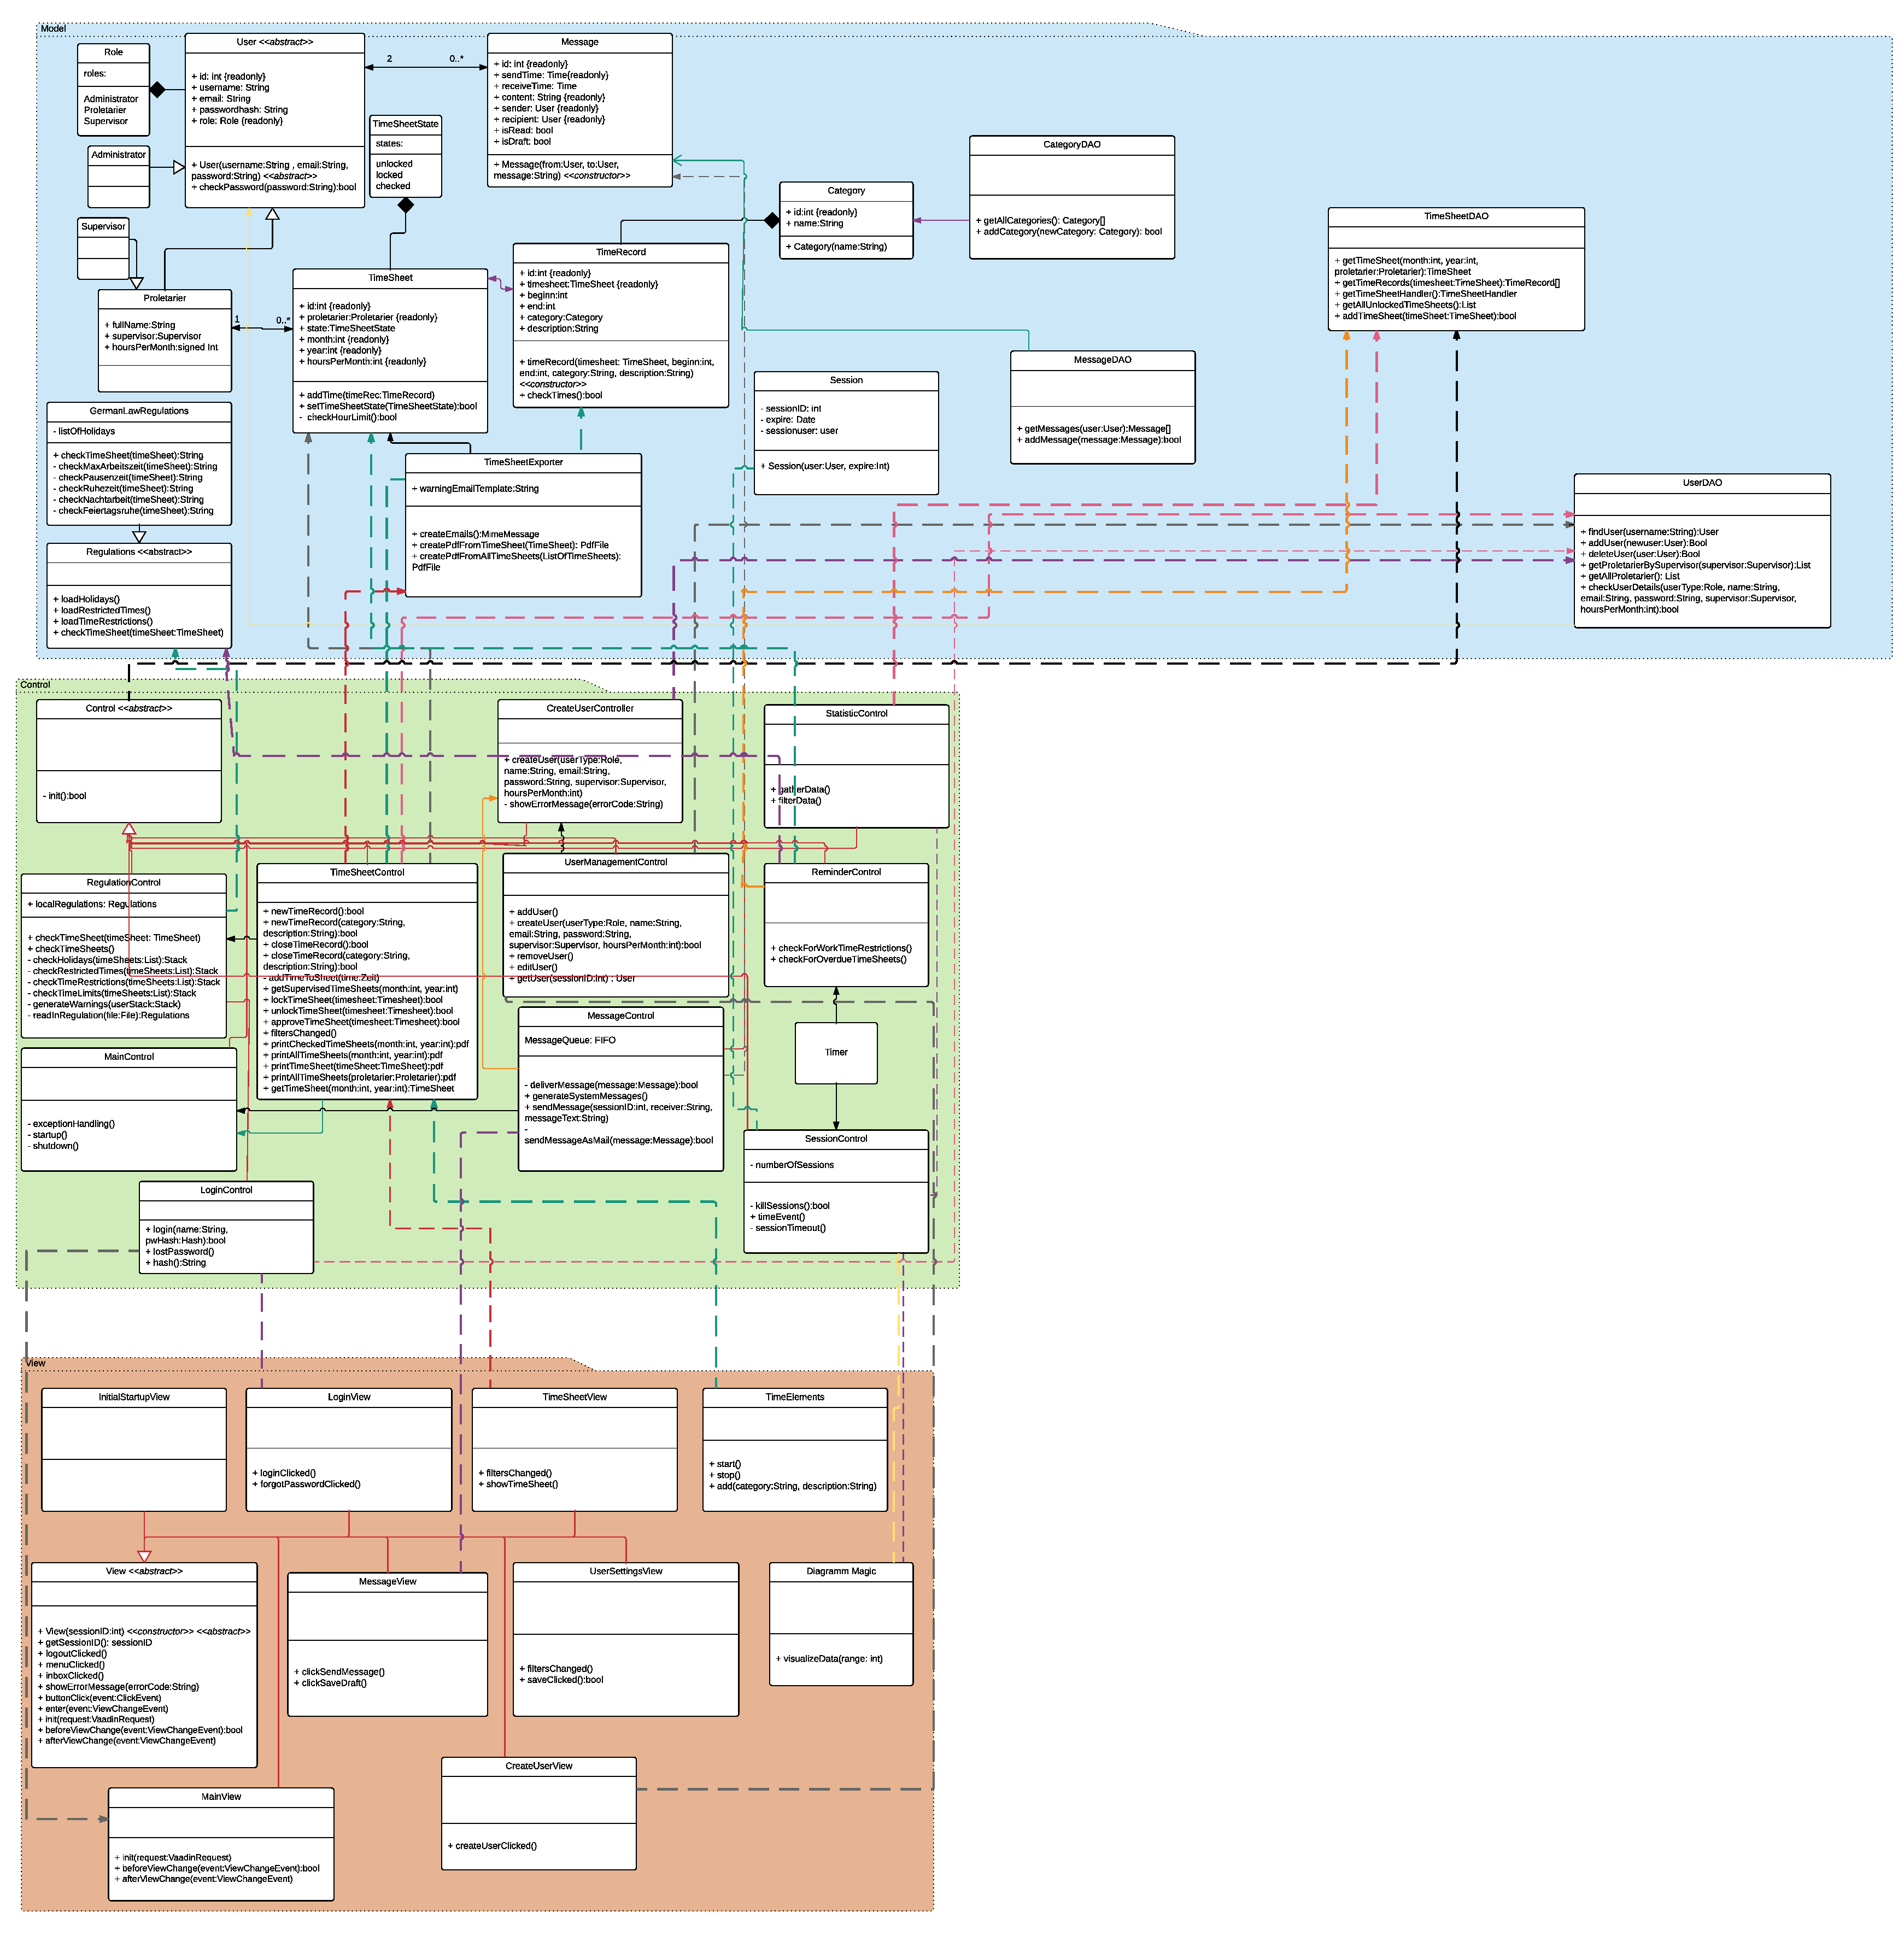
\includegraphics[width=\linewidth]{"Diagramms/class/overview.png"}\\
    \newpage
    \subsection{Model}
        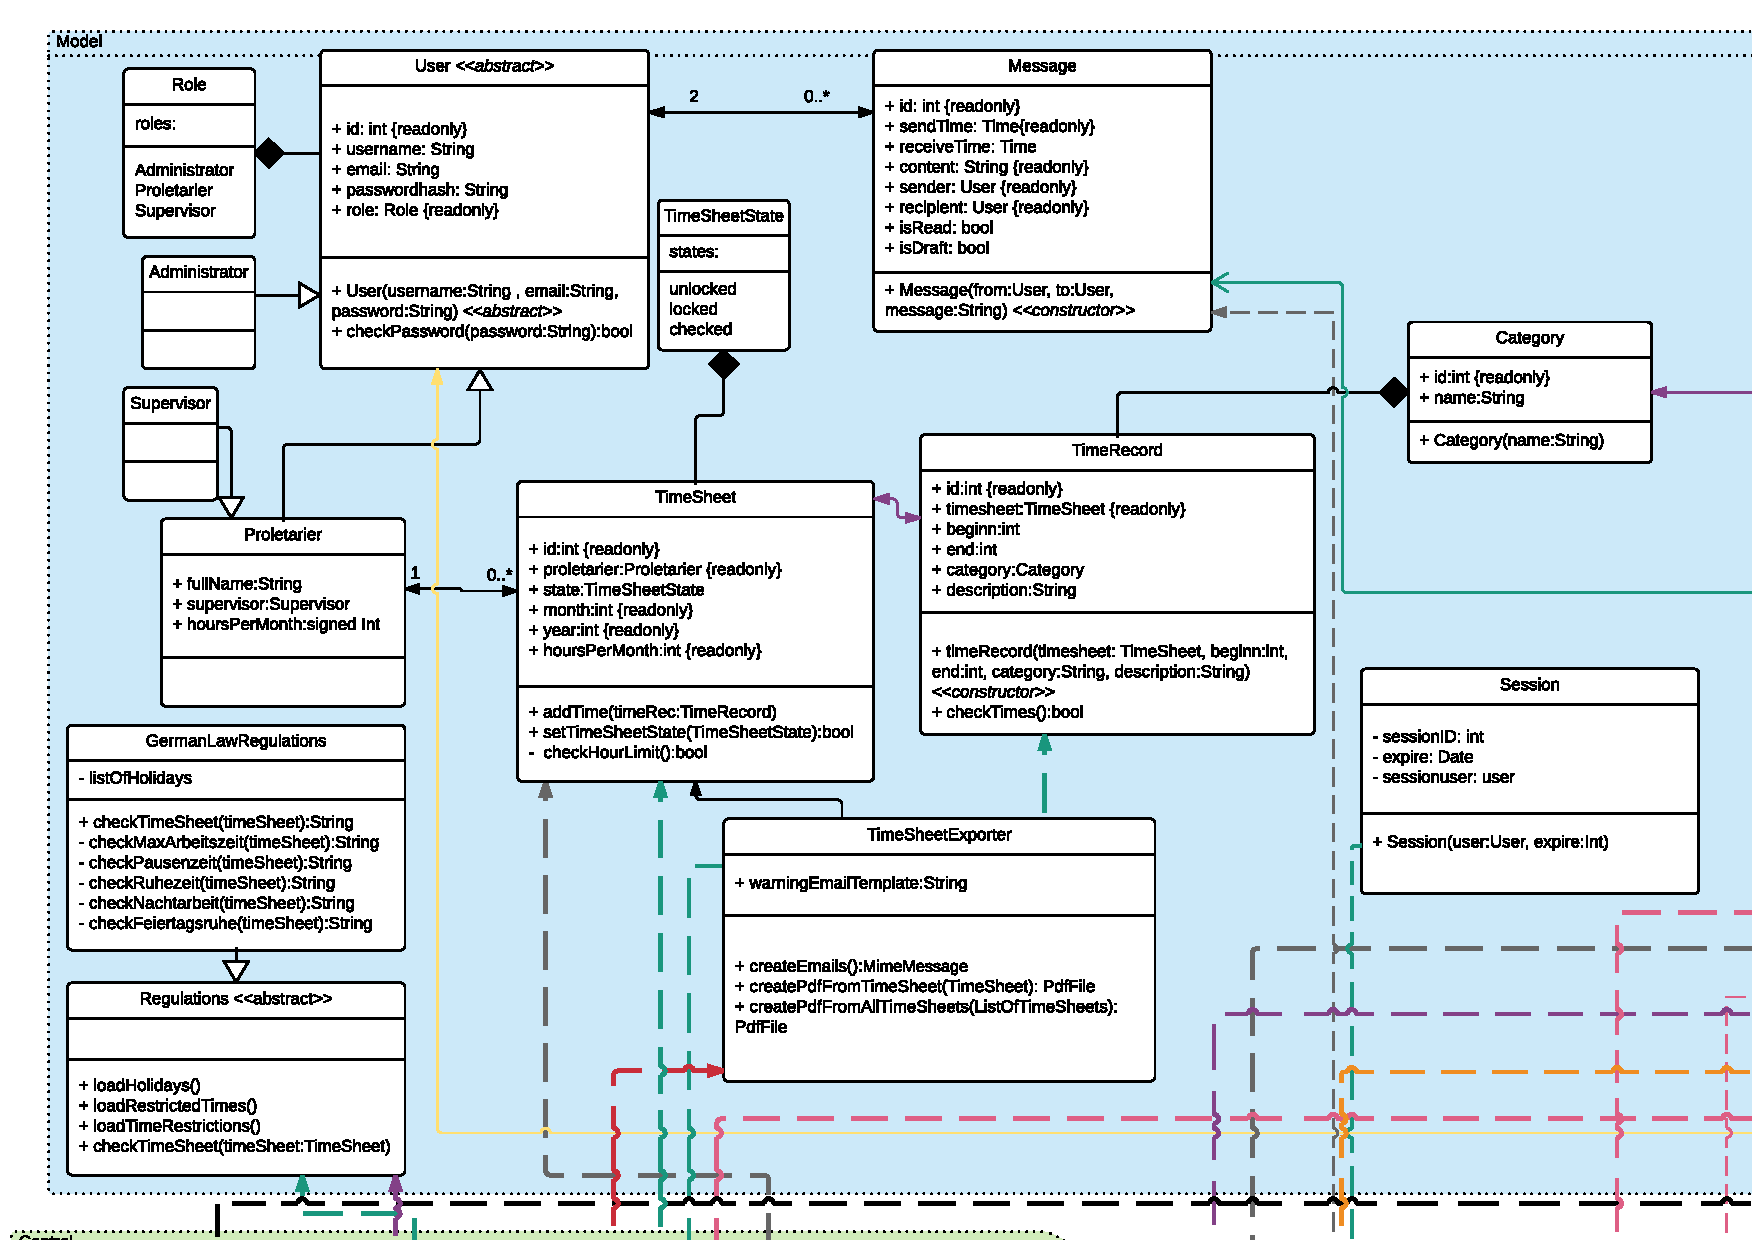
\includegraphics[width=\linewidth]{"Diagramms/class/model.pdf"}\\
        \begin{itemize}
            \item{Company}
                Speichert Informationen über die Firma in der die Zeiterfassung betrieben wird.
            \item{Entity}
                Grundform eines Benutzers, stellt grundlegende Daten und Funktionen für Spezialisierte Benutzer bereit.
                Folgende Spezialisierungen sind möglich:
                \begin{itemize}
                    \item{Admin}
                        Stellt Daten für und über den Admin bereit.
                    \item{User}
                        Stellt Daten für und über den User bereit, darüber hinaus hat der User eine verbing zu dem mit ihm assozierten Zeiterfassungen und Stundenzetteln.
                    \item{Supervisor}
                        Erweiterung des User um Gruppen von Usern zu verwalten.
                \end{itemize}
            \item{EntityCatalogue}
                Listet alle vorhanden Entities auf. Enthält Methoden um Entities hinzuzufügen, zu löschen oder zu verändern. Stellt darüber hinaus sicher, dass die alle einträge einzigartig sind.
            \item{Regulations}
                Lädt die gesetzlichen Regularien aus einer Datei und stellt diese für andere Klassen bereit.
            \item{TimeSheet}
                Speichert Zeiterfassungen. Methoden zur Validierung und sicherstellung der unveränderlichkeit sind vorhanden.
            \item{TimeSheetState}
                Zustände, die beschreiben, ob ein Stundenzettel verändert werden darf, bzw bereits überprüft wurde.
            \item{MonthAndYear}
                Klasse, die Zeitfunktionen für den Stundenzettel bereitstellt.
            \item{TimeRecord}
                Datenhaltung, der Zeiterfassung.
            \item{Session}
                Daten die mit einer Login Session assoziert sind(User, ablaufdatum, ...) werden in dieser Klasse gespeichert.
            \item{Category}
                Kategorie, die für die Zeiterfassung benötigt wird
            \item{Categories}
                Liste aller verfügbaren Kategorien.
            \item{Message}
                Nachrichten und damit Verbundene Metadaten können mit dieser Klasse erfasst werden.
            \item{HashThingy}
                Stellt Passwort Hash funktionen bereit.
            \item{TimeSheetToPdf}
                Klasse, um Stundenzettel als .pdf zu exportieren.
        \end{itemize}

    \subsection{Control}
        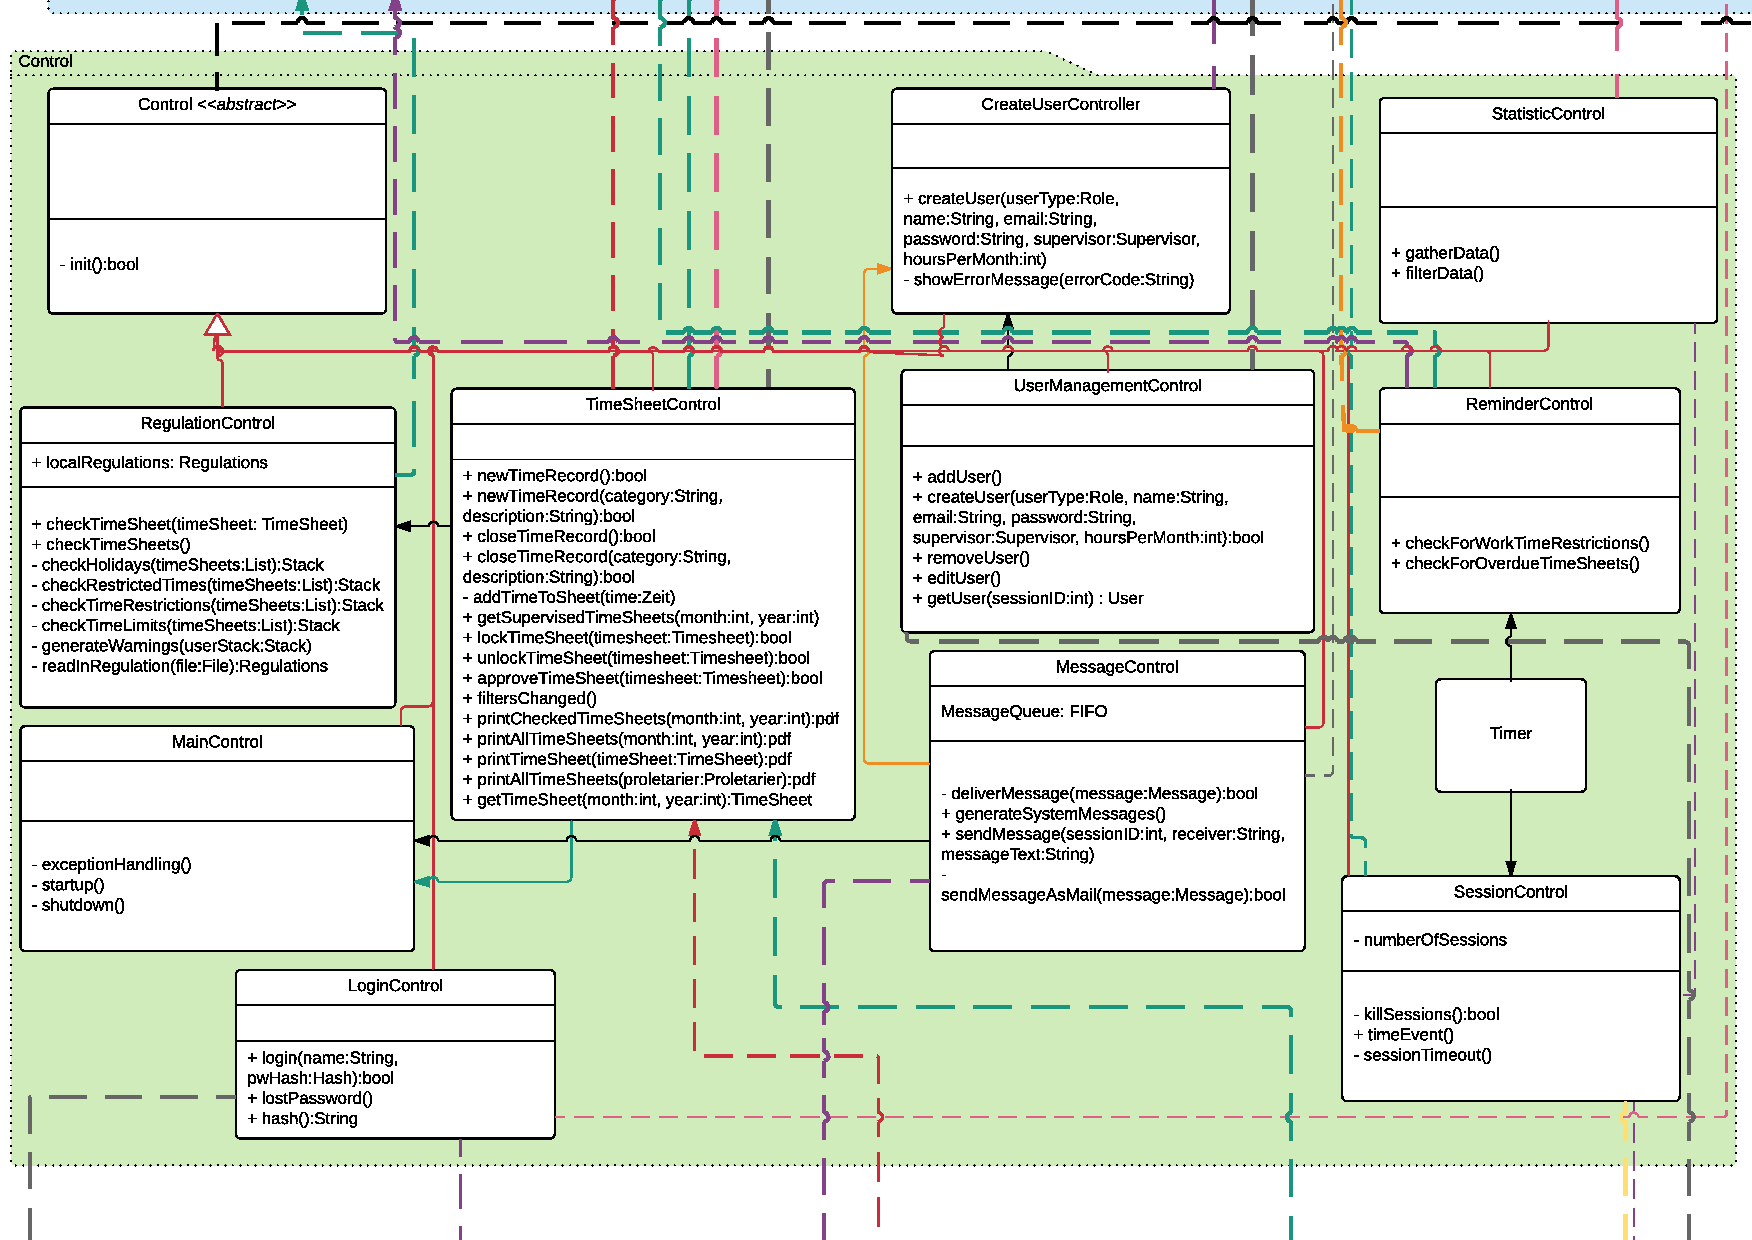
\includegraphics[width=\linewidth]{"Diagramms/class/control.pdf"}\\
        \begin{itemize}
            \item{Control}
                \begin{itemize}
                    \item{RegulationControl}
                       Überprüft Daten auf Gesetzeskonformität, leitet ebenfalls notwendige Schritte ein.
                    \item{MainControl}
                        Kontroliert den Hauptablauf des Programms.
                    \item{TimeSheetControl}
                        Regelt die Erstellung von Stundendaten für den Stundenzettel, darüber hinaus wird auch die abrarbeitung eines fertigen Stundenzettels geregelt.
                    \item{UserManagementControl}
                        Managed das hinzufügen, löschen und verändern von Benutzern
                    \item{LoginControl}
                        Überwacht das korrekte Einloggen von Benutzern.
                    \item{MessageControl}
                        Stellt Nachrichten zwischen Benutzern (und dem System) zu.
                    \item{StatisticControl}
                        Sammelt und generiert Statistiken über die erfassten Stundendaten.
                    \item{SessionControl}
                        Kontrolliert offene Sessions und terminiert diese nach ablauf eines gesetzen Zeitraums.
                \end{itemize}
            \item{Timer}
        \end{itemize}

    \subsection{View}
    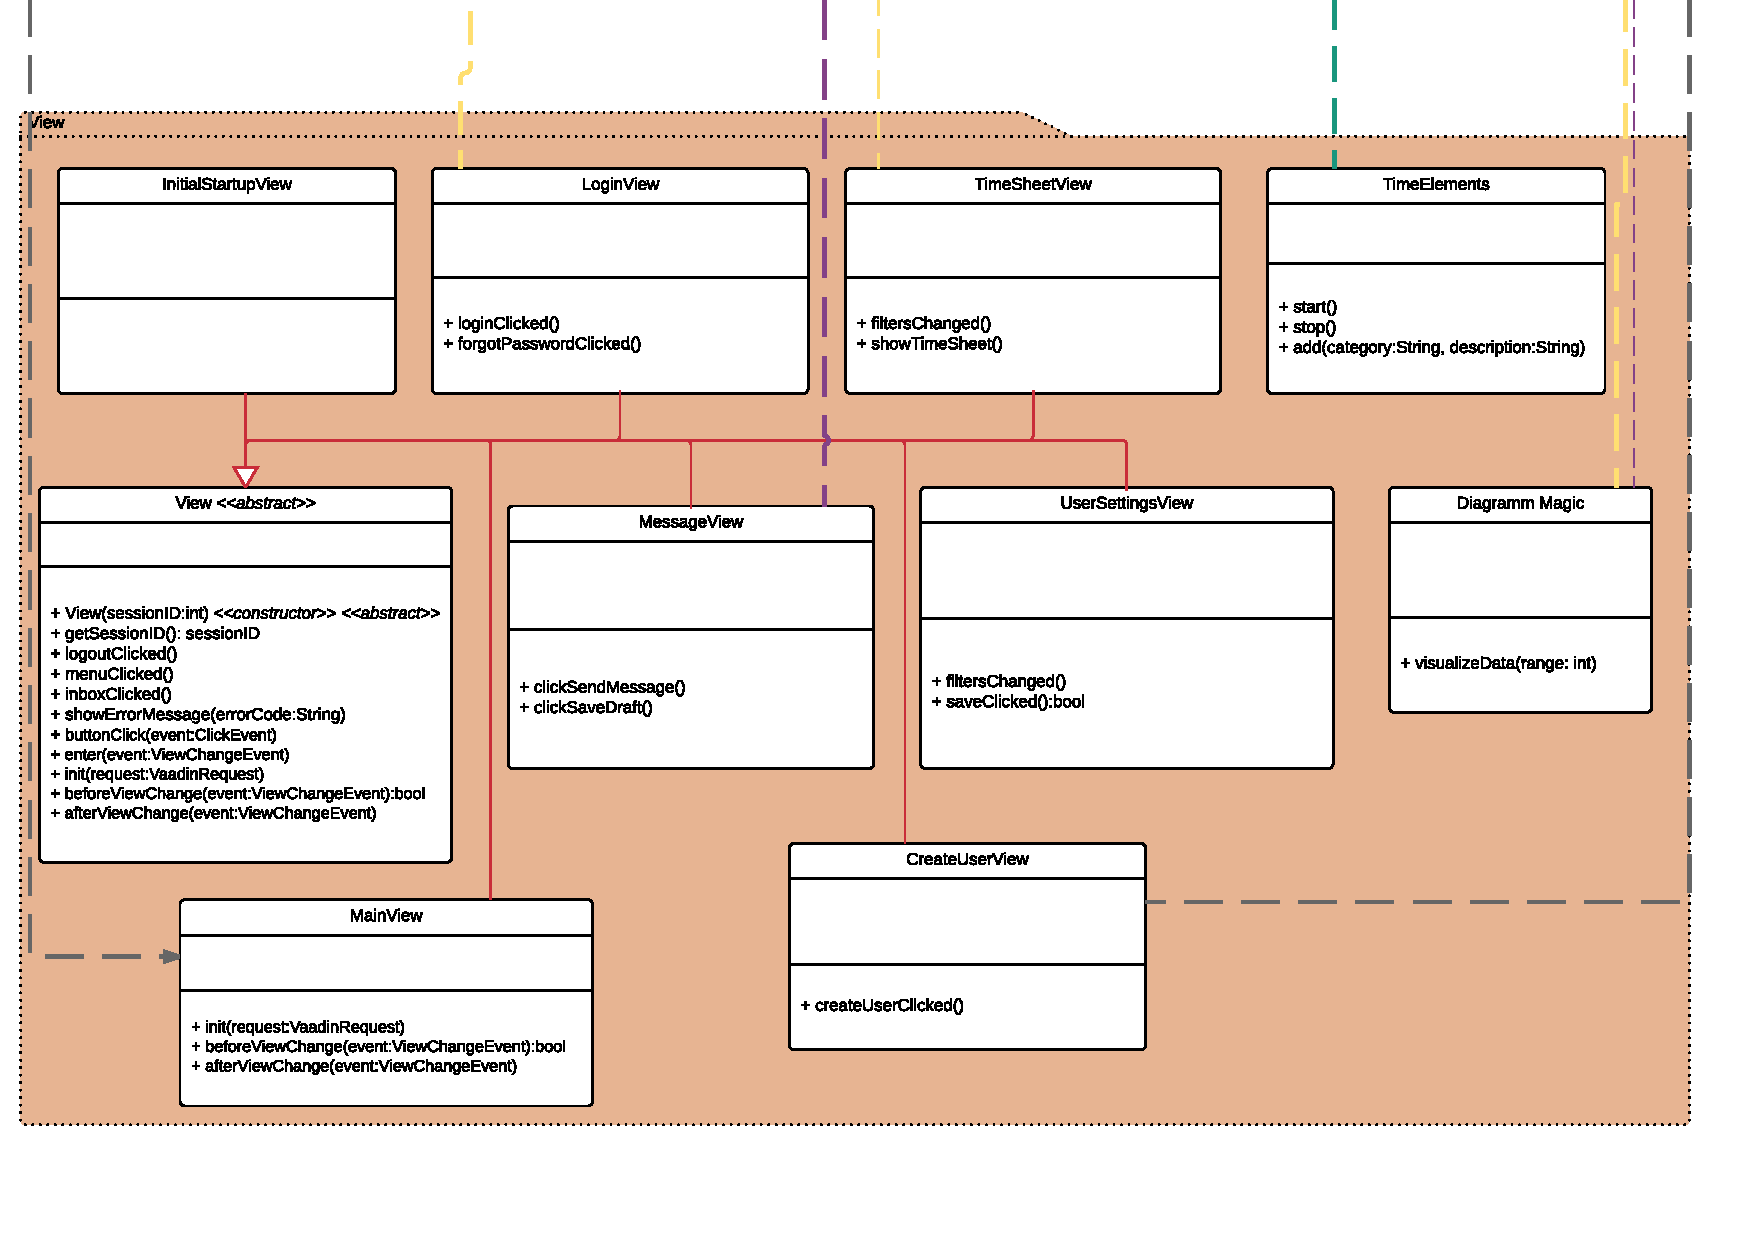
\includegraphics[width=\linewidth]{"Diagramms/class/view.pdf"}\\
        \begin{itemize}
            \item{View}
                \begin{itemize}
                    \item{LoginView}
                    \item{TimeSheetView}
                    \item{UserSettingsView}
                    \item{MainView}
                \end{itemize}
            \item{Diagramm Magic}
            \item{TimeElements}
        \end{itemize}
